\documentclass[titlepage]{jsreport}

\usepackage[dvipdfmx]{graphicx}
\usepackage[dvipdfmx]{color}
\usepackage{listings, jlisting}
\usepackage{cite}
\usepackage{url}
\usepackage{amssymb}
\usepackage{amsmath}



% ソースコードを挿入するための設定
\lstset{
language={Python},
basicstyle={\ttfamily\small},
backgroundcolor={\color[gray]{.95}},
keywordstyle={\color[rgb]{0.0,0.0,0.8}},
commentstyle={\color[rgb]{0.5,0.5,0.5}},
stringstyle={\color[rgb]{0.0,0.5,0.5}},
frame=single,
numbers=left,
numberstyle={\ttfamily\small},
breaklines=true,
breakindent = 10pt,
tabsize=2,
captionpos=t
}

\title{卒業論文のタイトル}
\author{慶應義塾大学理工学部物理情報工学科\\
指導教員 渡辺宙志\\
学籍番号 62116135\\
深瀬遥斗}
\date{2025年3月}

\begin{document}
\pagenumbering{roman}
\maketitle
\setcounter{tocdepth}{2}
\tableofcontents

\chapter{はじめに} \label{chap:introduction}
\pagenumbering{arabic}

「はじめに」もしくは「緒言」では、研究背景、目的、そして論文の構成を書く。第一章の前に目次をつける場合、目次のページ番号はi, ii,とローマ数字にして、本文からアラビア数字にするのが一般的だ。それを実現するため、\verb|\begin{document}|の直後にページ番号をローマ数字にするコマンド\verb|\pagenumbering{roman}|が、最初の\verb|\chapter|の後にアラビア数字にするコマンド\verb|\pagenumbering{arabic}|が挿入されている。

\section{研究の背景}

研究の背景は「なぜこの研究をしなければならないか」を、「大きい理由から小さい理由」へ書いていく。「大きい理由」は、「エネルギー問題」「安全」「便利」といった、「多くの人がほぼ納得するような理由」を挙げる。次に、その「大きな理由」を実現するために、これまでどのような試みがなされてきたかを説明する。これまでに読んだ論文のイントロダクションを参考に、必要な文献を引用しながら説得力のある文章を書くこと。

\section{研究の目的}

研究の背景を受けて、この研究分野は重要であるが、なんらかの不満点があることを述べる。その不満点は解決すべき問題であることを文献を引用しながら読者に納得させる。本研究の目的は、その不満点を解消することであることを述べ、その方法について簡単に述べる。

\section{本論文の構成}

論文の構成を説明する。まず本研究の目的を一行で書いてから、各章に何が書いてあるかを説明する。以下は例である。

\begin{quotation}
    本研究では、では、分野Aにおける手法Xの精度改善を行う。以下に本論文の構成を示す。第\ref{chap:introduction}章では、分野Aにおける手法の概観を紹介し、手法Xが広く用いられていることを示した。第\ref{chap:method}章では、本研究で用いる手法X、及びその改善手法であるX'について説明する。第\ref{chap:results}章では、本研究で提案した手法X'と、もととなった手法Xとの精度の比較を行う。第\ref{chap:summary}章では本研究で得られた知見を総括し、結論と今後の展望について述べる。
\end{quotation}

\chapter{原理} \label{chap:principle}

\section{市場の仕組み}
\subsection{売買契約の優先順位}
東証の取引所市場において売買立会による取引は,価格優先の原則と時間優先の原則に従い,競争売買によって行われる\cite{shokengaimuin}.
価格優先の原則とは,売呼値は低い値段の注文を,買呼値は高い値段の注文を優先して成立させるという取引上のルールである.
一方で時間優先の原則では,注文した時間の早かった注文が優先して成立されるが,時間優先の原則より価格優先の原則を先に適用させるため,時間優先の原則は同一値段の呼値に対してのみ適用される.
また,時間や価格に関係なく成行呼値は指値による呼値より優先される.

\subsection{板寄せとザラ場方式}
売買価格の決定方法には,始値や終値を定める場合に用いられる板寄せと,始値決定後の値段の決定に用いられるザラ場方式がある\cite{shokengaimuin}.

板寄せは図\ref{fig:opening}~(a)で示すように,売注文も買い注文も成行注文を優先して対当させる.
次に残りの成行注文と,指値注文を価格優先の原則に従って対当させていく.
最後に同じ呼値同士を時間優先の原則に従って対当させることで,図\ref{fig:opening}~(b)のようになり,始値は最後に対当させた価格である100となる.
また,ザラ場方式は図\ref{fig:opening}~(b)の状態から新たな注文を表に追加し,同様の優先順位に従って対当させていく.そのため,ザラ場での約定では,約定価格は必ずしも単一とは限らない.

\begin{figure}[htbp]
    \centering
    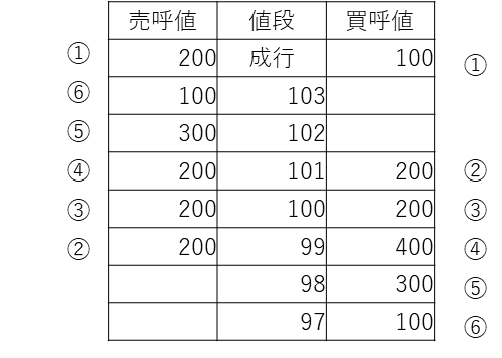
\includegraphics[width=0.49\linewidth]{fig/itayose.pdf}
    \hfil
    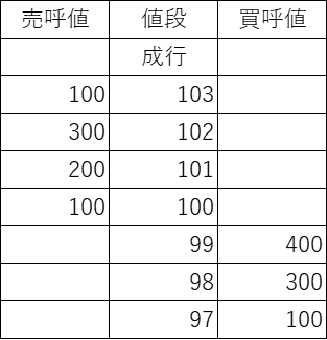
\includegraphics[width=0.335\linewidth]{fig/continuous.pdf}
    \caption{(a) 始値直前の板の状況.(b)始値直後の板の状況.}
    \label{fig:opening}
\end{figure}

\section{市場の性質}
\subsection{確率過程}
確率過程$W = (W_t)_{t \geq 0}$が次の性質1~4を満たすとき,確率過程$W$を標準ブラウン運動,あるいはウィナー過程という\cite{stochastic_integration}.
\begin{enumerate}
    \item $W_0 = 0  a.s.$
    \item 各$0 \leq s \leq t$に対して,$W_t - W_s \sim \mathcal{N}(0, t - s)$
    \item 独立定常増分糧である.
    \item 確率1で連続なパスを持つ.
\end{enumerate}

また,ある定数$\mu \in \mathbb{R}, \sigma > 0$とブラウン運動$W_t$を用いて表される確率微分方程式
\begin{equation}
    dS_t = \mu S_t dt + \sigma S_t dW_t \label{eq:geoBrow_equation}
\end{equation}

の解$S_t$は式(\ref{eq:geometric_Brown})で表され,この確率過程$S_t$を幾何ブラウン運動,$\sigma$をボラティリティという\cite{Stochastic_Calculus}.
\begin{equation}
    S_t = S_0 \exp{\left(\sigma W_t + \left( \mu - \frac{1}{2}\sigma^2 \right)t\right)} \label{eq:geometric_Brown}
\end{equation}

\subsection{ボラティリティ・クラスタリング}
? ボラティリティクラスタリングの説明を入れる

\subsection{ファット・テール}
図()で示すような,正規分布に比べて裾が厚く,べき乗測に従っている分布に対してファット・テールを持つという表現が用いられる(?参考文献を探す).
(?ファットテールの図を挿入)

べき分布の確率密度関数はある定数$a > 0,b > 0$を用いて式(\ref{eq:power_pdf})で表される\cite{PowerDistribution}.
\begin{equation}
    f(x) = \frac{ab^a}{x^{a + 1}} \qquad (x > b) \label{eq:power_pdf}
\end{equation}
よって相補累積分布関数$P(X \geq x)$は
\begin{equation}
    \begin{aligned}
        P(X \geq x) & = 1 - P(X \leq x)                     \\
                    & = 1 - \int_{b}^{x} f(t) \mathrm{d}t   \\
                    & = \frac{b^a}{x^a} \label{eq:survival}
    \end{aligned}
\end{equation}
となることより,べき分布の相補累積分布関数は両対数グラフで直線となる.そのため,ファット・テールを持つ分布の相補累積分布関数は図()のように両対数グラフで一部直線を持つ.
(?ファット・テールの相補累積分布関数の図を入れる)

\section{Zero-intelligence trader}
?ZItraderの説明を入れる

\subsection{Gode and Sunderモデル}
ZIトレーダーの1つにGodeとSunderによって提案されたモデルが存在する\cite{Gode_and_Sunder}.
以降このモデルをGode and Sunderモデルとする.
Gode and Sunderモデルは,市場規律による予算制約によって行動が制限されること\cite{market_displine}を用いて,ZIトレーダーに予算による制限を設けることで取引価格が均衡価格近傍に収束することや余剰をほぼ最大にするといった市場の特性を再現している.

はじめに各トレーダーには償却価値とコストが与えられ,$i$番目のトレーダーの償却価値を$v_i$,コストを$c_i$とする.
償却価値$v_i$とコスト$c_i$は$[1, V_{max}]$の整数の一様乱数に従って生成される.
次に,ランダムなトレーダーを選び確率1/2で売注文を,確率1/2で買注文を出す.
このとき,注文数は1株とし,呼値は売注文の場合は$[c_i, V_{max}]$で,買注文の場合は$[1, v_i]$でランダムとする.
ただし,$V_{max}$は一株当たりの注文価格の上限とする.
そしてこれまでの注文の記録と比較して,対当できるなら約定を成立させ,対当はできないが記録の中で最も取引が成立しやすい(売注文の場合は安く,買注文の場合は高い)価格である場合は新たにその価格を記録する.
以上の操作を全員が取引を行うか十分に時間が経過するまで繰り返すと,約定価格は図\ref{fig:gode_sunder_trade}の黒線のように変化する.
全トレーダーの呼値を,売注文の場合は昇順に,買注文の場合は昇順に並べることで図\ref{fig:gode_sunder_trade}の赤線と緑線のような需給曲線を引くことができ,約定価格が最終的に均衡価格近傍に収束している.
また,余剰についても需給曲線から求められる最大値の95 \%程度になっている.

予算制約を設けない完全にランダムなトレーダーと人間にも同様の実験を行ったところ完全にランダムなトレーダーのみ取引価格が均衡価格近傍に収束せず,余剰も9割を越えなかった.
そのため,Gode and Sunderモデルによってこれらの市場の特性が市場規律による予算制約によるものだと明らかにされている.
\begin{figure}[htbp]
    \centering
    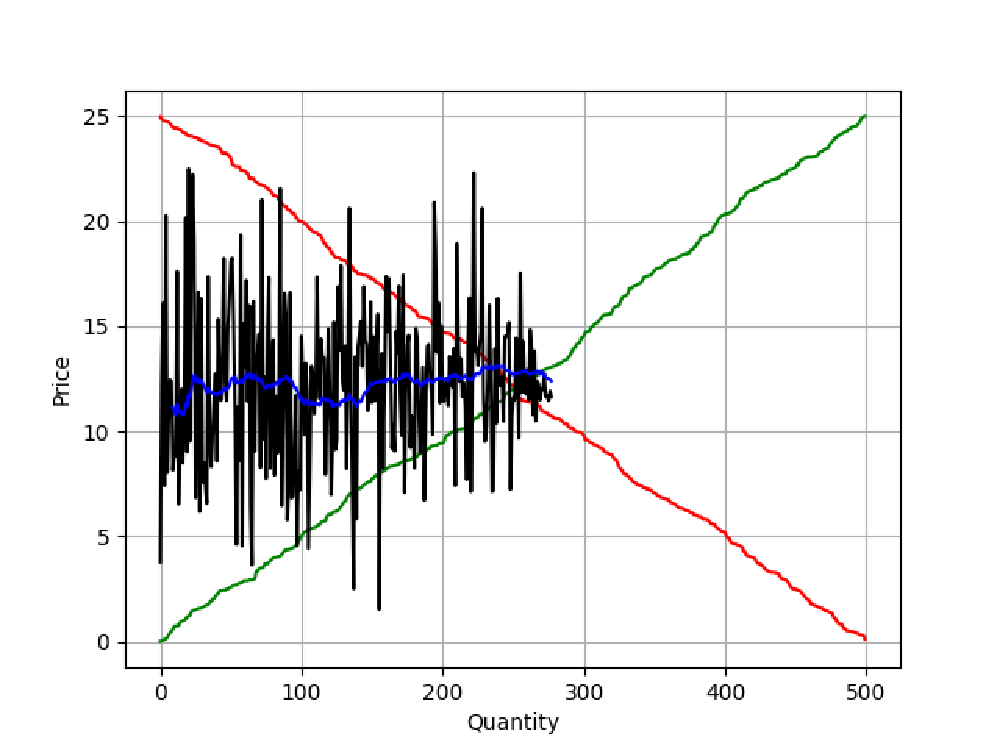
\includegraphics[width=10cm]{fig/gode_sunder_trade.pdf}
    \caption{Gode and Sunderモデルの需給曲線と取引価格.}
    \label{fig:gode_sunder_trade}
\end{figure}


\subsection{Genoaモデル}
Gode and Sunderモデルの他に,トレーダーの注文方法に制限を設け,更にクラスターを形成させることによって,ファット・テールとボラティリティ・クラスタリングを再現したモデルがある\cite{Genoa}.
以降,このモデルをGenoaモデルと呼ぶ.

前提として,トレーダーは限られた資産を用いて単一株を取引する.
また,トレーダーの人数を$N$人として,ステップ$h$における$i$番目のトレーダ-の全資産を$A_i(h)$,現金資産を$C_i(h)$,株価を$p(h)$とする.このとき,ステップ$h + 1$におけるトレーダー$i$の売呼値$s_i(h + 1)$を式(\ref{eq:Genoa_sell}),買呼値$b_i(h + 1)$を式(\ref{eq:Genoa_buy})で決定する.
\begin{equation}
    s_i(h + 1) = \frac{p(h)}{\mathcal{N}(\mu, \sigma_i)} \label{eq:Genoa_sell}
\end{equation}
\begin{equation}
    b_i(h + 1) = p(h) \mathcal{N}(\mu, \sigma_i) \label{eq:Genoa_buy}
\end{equation}
ただし,$\mathcal{N}(\mu, \sigma_i)$は平均$\mu = 1.01$,標準偏差$\sigma_i$のガウス分布から生成される乱数で,$\sigma_i$は定数$k = 3.5$,時間窓数$T_i = 20$,過去$T_i$間におけるボラティリティ$\sigma(T_i)$を用いて式(\ref{eq:Genoa_sigma_i})で定義される.
\begin{equation}
    \sigma_i = k \sigma(T_i) \label{eq:Genoa_sigma_i}
\end{equation}

また,ステップ$h + 1$におけるトレーダー$i$の売注文の株数$a_i^s$を式(\ref{eq:Genoa_a_i^s}),買注文の株数$b_i^s$を式(\ref{eq:Genoa_a_i^b})に従って決定する.ただし,$r_i$は$[0, 1]$の一様乱数である.
\begin{equation}
    a_i^s = \lfloor r_i A_i(h) \rfloor \label{eq:Genoa_a_i^s}
\end{equation}
\begin{equation}
    a_i^b = \left\lfloor \frac{r_i C_i(h)}{b_i} \right\rfloor \label{eq:Genoa_a_i^b}
\end{equation}

Gode and Sunderモデルと同様に全トレーダーの呼値を,売注文の場合は昇順に,買注文の場合は昇順に並べることで需給曲線が得られる.
均衡価格$p^*(h)$は需要曲線と供給曲線の交点として,板寄せと同様の取引方法を用いて,均衡価格$p^*(h)$より安い売呼値と高い買呼値を全て価格$p^*(h)$で売買を成立させる.
そのため
\begin{equation}
    p(h + 1) = p^*(h) \label{eq:Genoa_price}
\end{equation}
となる.
ただし,同じ呼値同士は時間優先の原則ではなく,完全にランダムな優先順位で対当させる.

注文は,基本的には確率1/2で売注文,確率1/2で買注文となるが,クラスターに属している場合は例外が発生する.

各ステップにおいて,すべてのトレーダーのペアについて,確率$P_a$で2人のトレーダー間にクラスターが形成される.
そのため,クラスターはステップが進むにつれて成長や合併を行う.
また,各ステップで確率$P_c$で1つのクラスターをアクティブに,確率$1 - P_c$ですべてのクラスターをインアクティブにする.
アクティブになったクラスターのトレーダーは,全員の出す注文の種類(売注文か買注文か)が同じになり,取引後にクラスターを消滅させる.

?クラスターの図を入れられたら入れる





\chapter{手法} \label{chap:method}
\section{Gode and Sunderモデルの解析}
本研究では,はじめにGode and Sunderモデルのトレーダーの資産が幾何ブラウン運動に従っているか,LeBaronらによって作成されたGode and Sunderモデルのコード\cite{Gode_and_Sunder_code}をもとに解析をおこなった.

\subsection{Gode and Sunderモデルの設定}
LeBaronらのコードでは取引期間が1期間のみであったため,取引期間$T$を新たに追加して,複数期間にわたって取引が行うことができるように変更した.
また,トレーダーが1期間に売注文と買い注文を1回ずつの最大2回取引を行うことができたので,売注文か買注文のいずれかを最大1回のみ出すことができるように変更をおこなった.
更に,各トレーダーに資産の項目を追加した.
トレーダーの人数を$N$人として,期間$h$における$i$番目のトレーダーの資産を$A_i(h)$,取引価格を$p(h)$で表し,売注文が成立した場合は式(\ref{eq:Gode_asset_sell}),買い注文が成立した場合は式(\ref{eq:Gode_asset_buy})のように資産を変動させた.
\begin{equation}
    A_i(h + 1) = A_i(h) + p(h) \label{eq:Gode_asset_sell}
\end{equation}
\begin{equation}
    A_i(h + 1) = A_i(h) - p(h) \label{eq:Gode_asset_buy}
\end{equation}
このとき,$A_i(h + 1)$が負の値をとることを許した.

シミュレーションに用いたパラメータを表\ref{tbl:Gode_param}に示す.

\begin{table}[htbp]
    \begin{center}
        \caption{Gode and Sunderモデルの解析で用いたパラメータ}
        \begin{tabular}{lr}
            \hline\hline
            トレーダーの人数 $N$          & 2000 \\
            期間 $T$                      & 100  \\
            呼値の上限 $V_{max} $         & 25   \\
            トレーダーの初期資産 $A_i(0)$ & 500  \\ \hline
            \label{tbl:Gode_param}
        \end{tabular}
    \end{center}
\end{table}

以上のシミュレーションを,それぞれの期間において償却価値$v_i$とコスト$c_i$を変化させる場合と変化させない場合について資産分布と資産変動の解析をおこなった.

\subsection{Gode and Sunderモデルの解析方法}
トレーダーの資産分布と資産変動がファット・テールになっているか,相補累積分布関数を作成して標準正規乱数の相補累積分布関数と比較した.

資産分布は,まずトレーダーの最終的な資産$A_1(T), A_2(T), ..., A_N(T)$について平均$\mu_A$と標準偏差$\sigma_A$を求め,式(\ref{eq:normalization})に従って標準化された資産$\tilde{A_1}, \tilde{A_2}, ..., \tilde{A_N}$を得た.
\begin{equation}
    \tilde{A_i} = \frac{A_i(h) - \mu_A}{\sigma_A} \label{eq:normalization}
\end{equation}
次に,$N$個の標準正規乱数$Z_1, Z_2, ..., Z_n$を用意し,$\tilde{A_1}, \tilde{A_2}, ..., \tilde{A_N}$と$z_1, z_2, ..., z_n$に対して絶対値をとり,それぞれの相補累積分布関数の両対数グラフの比較をおこなった.

資産変動は,トレーダー$i$の資産$A_i(1), A_i(2), ...A_i(T)$について,取引を行われていない,つまり$A_i(h) = A_i(h + 1)$の場合は$A_i(h + 1)$を除外した新たな資産変動のリスト$A_i(1)', A_i(2)', ...A_i'(T')$を作成した.次に式(\ref{eq:asset_return})に従って資産の変動の割合$r_i(1), r_i(2), ..., r_i(T' - 1)$を求め,資産$A_1(T), A_2(T), ..., A_N(T)$と同様の手順で標準正規乱数との相補累積分布関数の両対数グラフの比較をおこなった.
\begin{equation}
    r_i(h) = \frac{A_i(h) - A_i(h - 1)}{A_i(h - 1)} \label{eq:asset_return}
\end{equation}




\chapter{結果} \label{chap:results}

\section{図の入れ方}

図は、数が多くなければとりえあずfigといったディレクトリにまとめて入れておくと良いだろう。数が増えてきて管理が難しくなったら節ごとにわけるなど工夫すること。画像ファイルは原則としてPDFにすること。例えば\verb|temperature.pdf|を入れたいなら、

\begin{lstlisting}[language={[LaTeX]TeX}]
\begin{figure}[htbp]
    \centering
    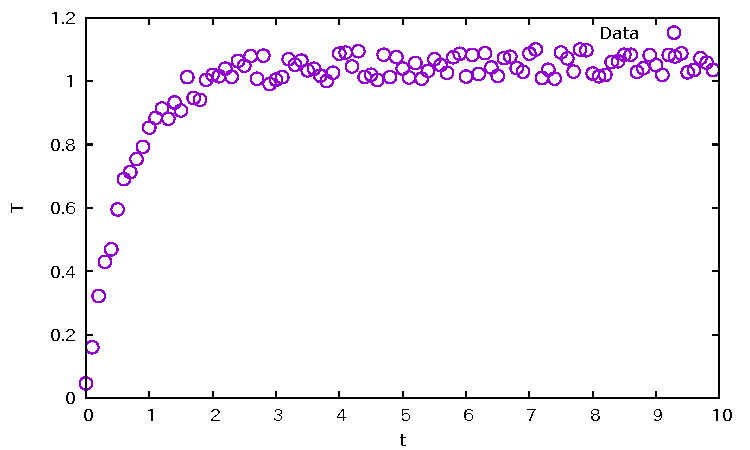
\includegraphics[width=0.49\linewidth]{fig/temperature.pdf}
    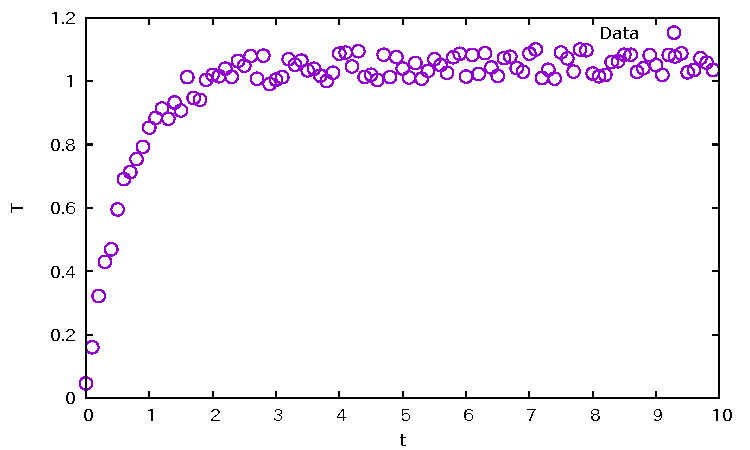
\includegraphics[width=0.49\linewidth]{fig/temperature.pdf}
    \caption{温度の時間発展。}
    \label{fig:temperature}
\end{figure}

\end{lstlisting}

とすると、以下のような図が得られる。
\begin{figure}[htbp]
    \centering
    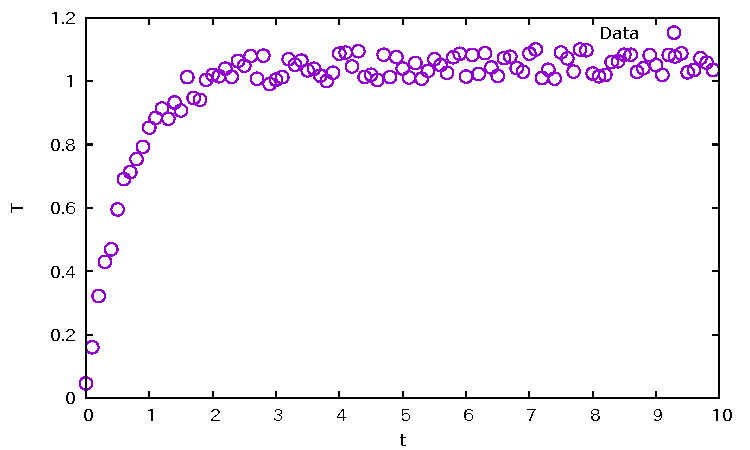
\includegraphics[width=0.49\linewidth]{fig/temperature.pdf}
    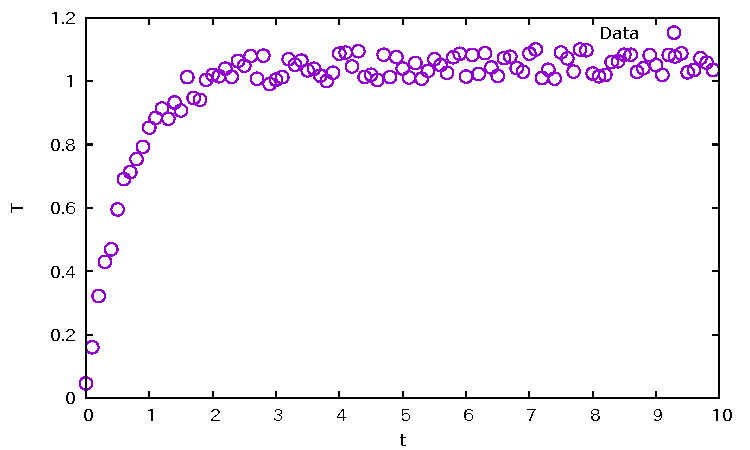
\includegraphics[width=0.49\linewidth]{fig/temperature.pdf}
    \caption{温度の時間発展。}
    \label{fig:temperature}
\end{figure}

この時、元データと、データからPDFを作るためのプロットファイルもしくはスクリプトファイルを一緒に入れておく。この時、画像ファイルとプロットファイルの名前を同じにしておくと良い。例えばgnuplotを使って\verb|temperature.pdf|という画像を作るなら、プロットファイルを\verb|temperature.plt|にしておく。すると、

\begin{lstlisting}[language=bash]
gnuplot temperature.plt
\end{lstlisting}

を実行することで\verb|temperature.pdf|ができるのでわかりやすい。

また、名前を揃えておくとmakefileとの相性が良くなる。例えば\verb|pressure.pdf|、\verb|temperature.pdf|、\verb|error.pdf|の三つのファイルが、同名のpltファイルから作成されるなら

\lstinputlisting[language=make]{fig/makefile}

といったmakefileを作っておけば、make一発で三つのファイルを作ることができるので便利だ。

もちろんPythonのMatplotlibを使っても良いが、いずれにせよ「データとスクリプトからコマンド一発で図のファイルが作成できる状況にしておく。

\chapter{考察および結論} \label{chap:summary}

考察は、「研究の背景」及び「目的」において提起した問題に正しく答えるようにする。得られた結果は満足すべきものだったか?不満があるならその理由はなにか?解決できそうなのか?また、「大きい理由」にも言及する。本研究によりどのような課題が見つかったかを書き、この分野における「研究の流れ」においてのような位置づけにあるかを説明した上で、今後、どのような発展の方向があるかについて書く。

\chapter*{謝辞}
はじめに指導教員である渡辺宙志先生にお礼申し上げます.
金融という物理情報工学科に関連のない分野にもかかわらず,研究の方向性や方法など様々な助言を送っていただいたことや,プログラミングやソフトウェアの知識に疎い私に対して丁寧に指導していただいたことなど,これらの貴重なアドバイスや指導が私の研究や成長に大いに役に立ちました.


また,研究室ミーティングや練習発表会で質問や助言を与えてくださった先輩方にも感謝しております.
特に,研究室でお会いする機会の多かった小林さんと竹内さんからは,研究への取り組み方だけでなく,自身が関心を抱く分野への取り組み方について,多くのことを学ばせていただきました.

そして,研究室の同期の皆さんにも感謝しております.
中でも伊藤君は機械の操作方法やハンズオンの内容が理解できていなかった私に対して,その都度アドバイスをくれました.
現在,私が問題なく研究を継続できているのは,伊藤君のおかげです.

最後に,これまで私を支えてくれた両親に心よりお礼申し上げます.
本研究に取り組むことができたのは,大学進学や日常生活において自由な選択肢を与え、それらを支えてくれた両親のおかげです.
ありがとうございました.

\appendix

\chapter{ソースコード}

\lstinputlisting[caption = 適当なPythonスクリプト, label = prog:sample]{src/sample.py}

\bibliographystyle{junsrt}
\bibliography{reference}

\end{document}
